%%=============================================================================
%% Push-notificaties
%%=============================================================================

\chapter{Notificaties}%
\label{ch:notificaties}

In dit hoofdstuk gaan we de lokale notificaties van native en cross-platform vergelijken. 
Met deze resultaten kunnen we dan een gepaste conclusie vormen.

\section{Native}
\subsubsection{Wat hebben we nodig}
%tools, libraries, ...
Om lokale notificaties aan te kunnen maken bij Android maken we gebruik van de NotificationCompat API aangeboden 
door de Android support library. Deze stelt ons in staat om de titel, tekst, pictogram en andere inhoud van de 
notificatie in te stellen. Notificaties kunnen ook worden ingesteld om speciale acties te ondernemen bij het openen 
van de applicatie via de notificatie. Er kan ook een eventueel een prioriteit worden meegegeven.

\subsubsection{Uitvoering}
\paragraph{1. Dependancy toevoegen}
Normaal zijn bevatten alle projecten gestart met Android Studio de nodige dependancies om de NotificationCompat API
te gebruiken. Maar voor de zekerheid verifiëren we dat onderstaande dependancy er bij zit.
\begin{minted}{java}
  val core_version = "1.6.0"
  dependencies {
      implementation("androidx.core:core-ktx:$core_version")
  }
\end{minted}
Als de dependancy is toegevoegd dan kunnen we notificaties beginnen aanmaken.

\paragraph{2. Notificatie aanmaken}
Een notificatie wordt aangemaakt met het NotificationCompat.Builder object. 
\begin{minted}{kotlin}
   var builder = NotificationCompat.Builder(this, CHANNEL_ID)
    .setSmallIcon(DRAWABLE_ICON)
    .setContentTitle(TITLE)
    .setContentText(DESCRIPTION)
    .setPriority(NotificationCompat.PRIORITY_DEFAULT)
\end{minted}
\begin{figure}[H]
    \centering
    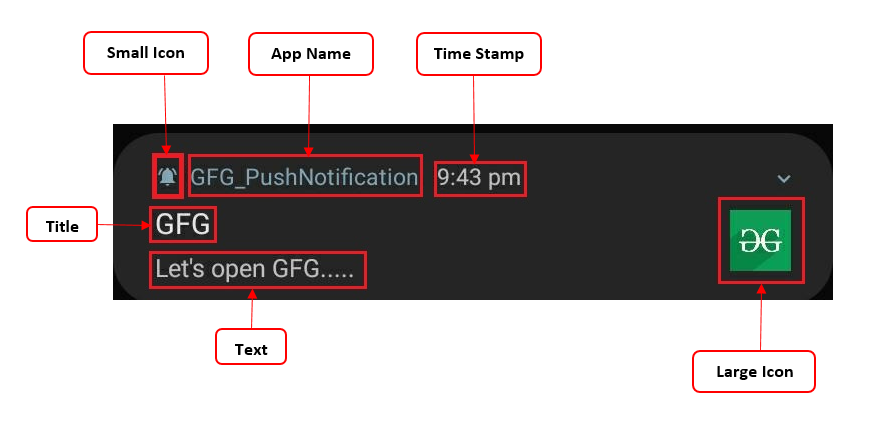
\includegraphics[height=0.5\textheight]{NotificationAnatomy.png}
    \caption{Anatomy standaard notificatie .}% TODO \parencite{https://www.geeksforgeeks.org/how-to-push-notification-in-android/}
\end{figure}

\paragraph{3. Channel aanmaken}
Het laatste dat we nodig hebben vooraleer de notificatie getoond kan worden is een channel. Deze worden 
gebruikt om notificaties te groeperen volgens hun belang. Om een channel aan te maken gebruiken we 
de .createNotificationChannel() methode. Het maakt niet uit wanneer of waar deze code wordt uitgevoerd. 
Het is enkel belangrijk dat de channel wordt aangemaakt vooraleer er wordt geprobeerd om notificaties 
te tonen.
\begin{minted}{kotlin}
private fun createNotificationChannel() {
  // Channel aanmaken
  val channel = NotificationChannel(CHANNEL_ID, CHANNEL_NAME, NotificationManager.IMPORTANCE_DEFAULT).apply {
      description = CHANNEL_DESCRIPTION
  }
  // Channel bij het systeem registreren
  val notificationManager: NotificationManager =
      getSystemService(Context.NOTIFICATION_SERVICE) as NotificationManager
  notificationManager.createNotificationChannel(channel)
}
\end{minted}

\paragraph{4. Actie toevoegen}
Als onderdeel van de performantie te testen, zullen we de notificaties instellen om niet het hoofdscherm, 
maar een ander scherm te tonen bij het openen van de applicatie via de notificatie. Dit kunnen we doen met 
de Intent en PendingIntent objecten. Aan het Intent object kunnen acties worden meegegeven. Hier wordt er 
gespecificeerd welk scherm en welke actie er moet gebeuren. Daarna wordt het Intent object aan het PendingIntent 
object meegegeven dat op zijn beurt wordt meegegeven aan de .setContentIntent(PENDINGINTENT) methode.
\begin{minted}{kotlin}
  Intent intent = new Intent(context, SpecifiekSchermActivity.class);
  intent.setAction("ACTION_MY_ACTION");
  PendingIntent pendingIntent = PendingIntent.getActivity(context, 0, intent, PendingIntent.FLAG_UPDATE_CURRENT);

  var builder = NotificationCompat.Builder(this, CHANNEL_ID)
    .setSmallIcon(DRAWABLE_ICON)
    .setContentTitle(TITLE)
    .setContentText(DESCRIPTION)
    .setPriority(NotificationCompat.PRIORITY_DEFAULT)
    .setContentIntent(pendingIntent) // Voeg deze toe
\end{minted}

\paragraph{5. Notificatie tonen}
Tot slot kunnen we dan de notificatie tonen met de .notify() methode van de NotificationManagerCompat. 
Eerst wordt de notificationManager aangemaakt waarna de notificatie wordt getoond.
\begin{minted}{kotlin}
  NotificationManagerCompat notificationManager = NotificationManagerCompat.from(context);
  notificationManager.notify(notificationId, builder.build());
\end{minted}

\subsubsection{Ontwikkeltijd}

\paragraph{Geïnvesteerde tijd}

\paragraph{Compiletijd}

\subsubsection{Performantie}

\subsubsection{Schaalbaarheid}

\subsubsection{Conclusie}


\section{Cross-platform}
\subsubsection{Wat hebben we nodig}
%tools, libraries, ...
Om lokale notificaties bij React native te tonen gaan we gebruik maken van de externe library Notifee.



\subsubsection{Uitvoering}

\subsubsection{Ontwikkeltijd}

\paragraph{Geïnvesteerde tijd}

\paragraph{Compiletijd}

\subsubsection{Performantie}

\subsubsection{Schaalbaarheid}

\subsubsection{Conclusie}






















